\chapter[Self-Organizing Map for High-Redshift Galaxies]{Results of Training High-Redshift Galaxies for One-Dimensional Self-Organizing Maps}
\pagestyle{plain}
\label{app: high_Z_1d_soms}
\myappendices

As mentioned in Section~\ref{sec: 1D_somz}, we changed the size of the SOM from $1\times2$ to $1\times22$. In that section we show some example of the results, here we show the rest of the maps to monitor the changes in the map in various sizes.

\label{app: 1d}
    \begin{figure}
        \begin{subfigure}[b]{0.5\textwidth}
            \centering
            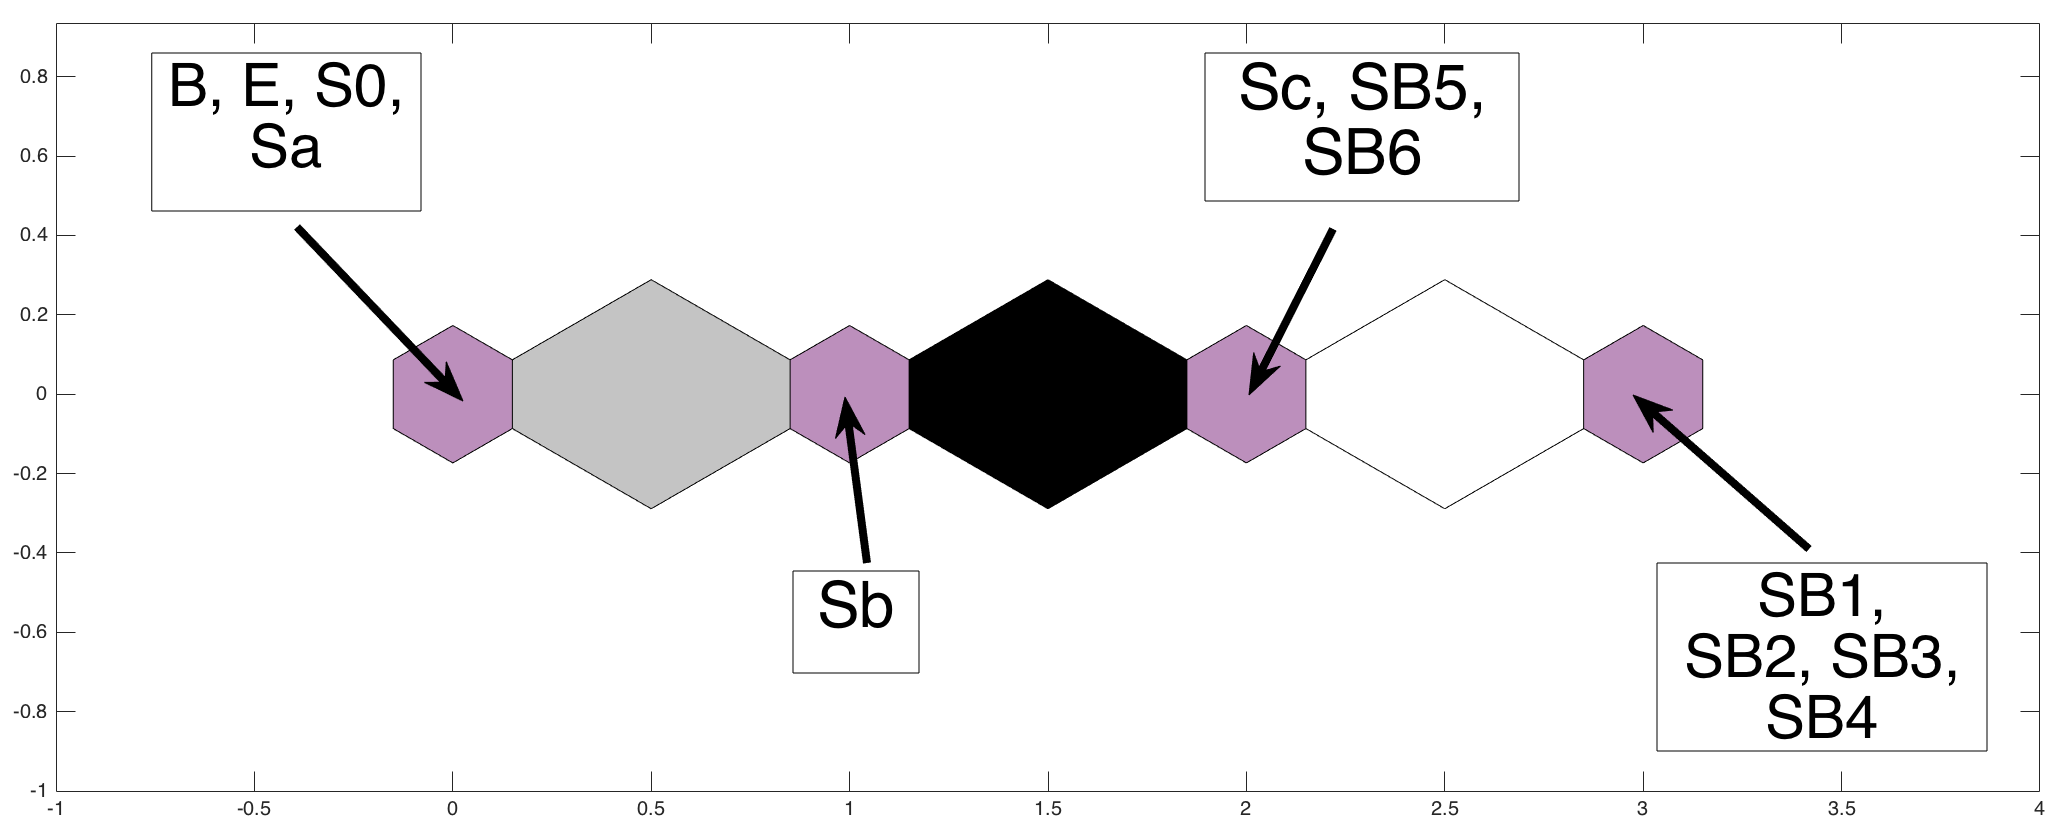
\includegraphics[width=\textwidth]{../image_paper2/1d/apps/dist_1_by_4.png}
            %\caption{$1\times4$ weight map}
             %\label{fig: 1by4T}
        \end{subfigure}
        \hfill
        \begin{subfigure}[b]{0.5\textwidth}
             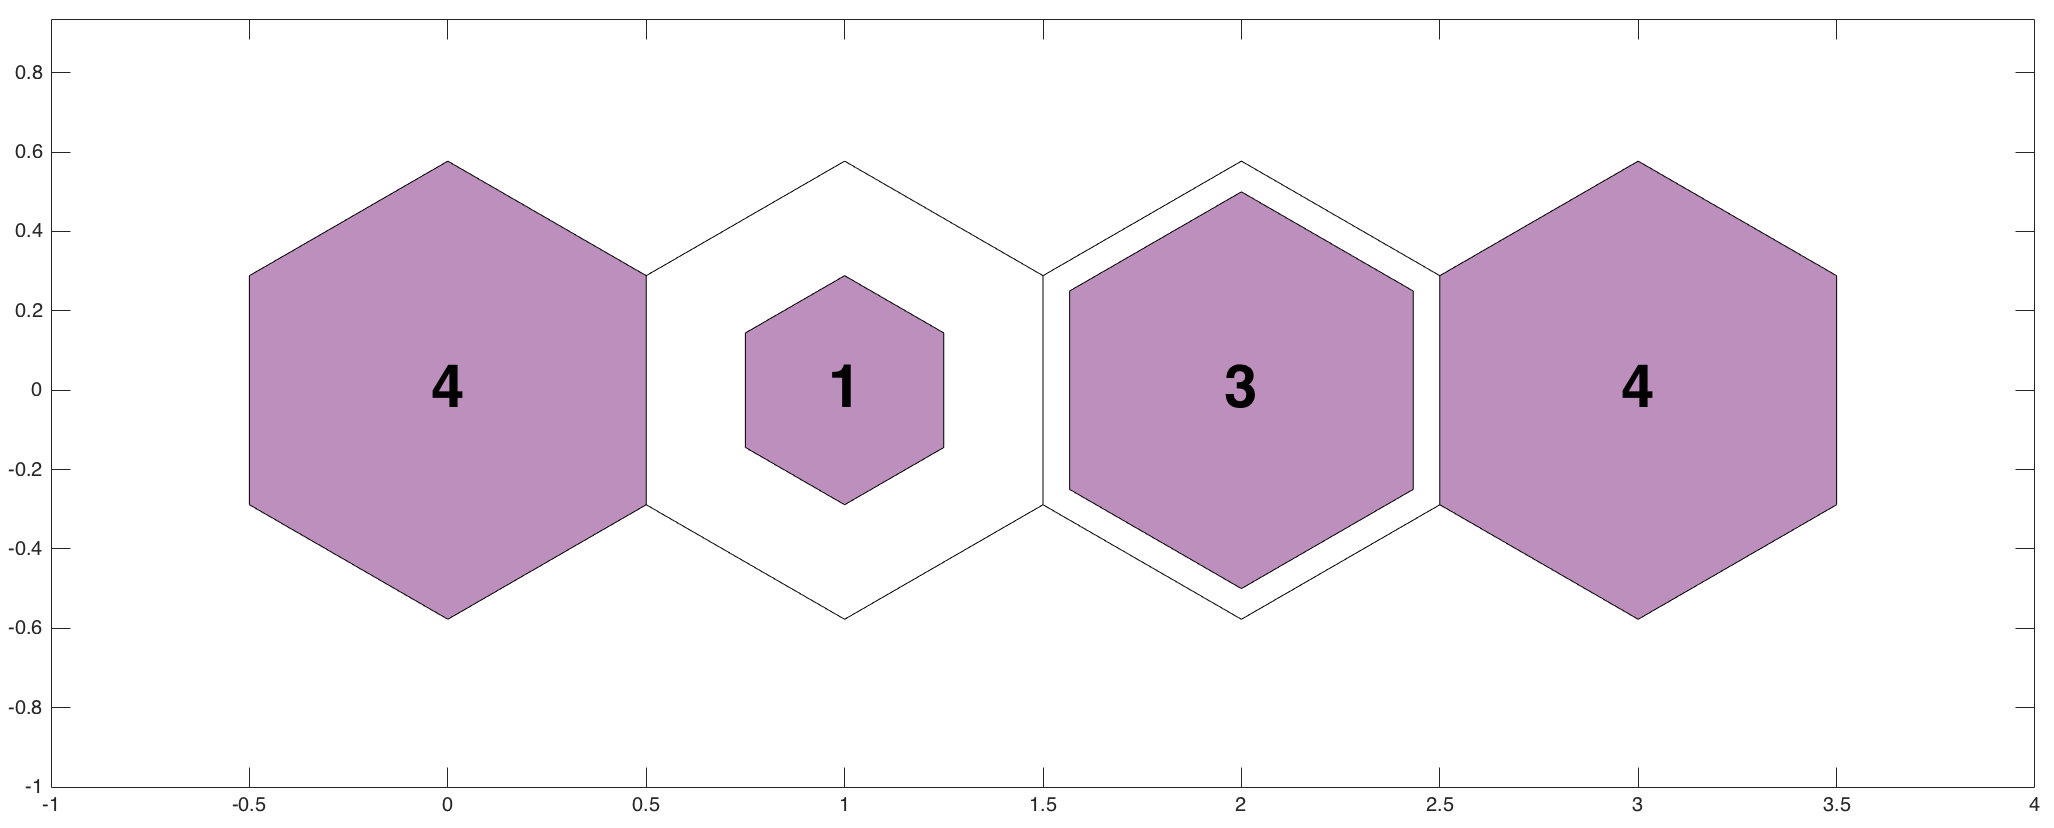
\includegraphics[width=\textwidth]{../image_paper2/1d/apps/hit_t_1_by_4.png}
             %\caption{$1\times4$ hits map}
             %\label{fig: 1by4Thits}
        \end{subfigure}
                \caption{Results of training network in $1\times4$~grid.}
         \label{fig: 1by4T}
    \end{figure}
    
    \begin{figure}
        \begin{subfigure}[b]{0.5\textwidth}
            \centering
            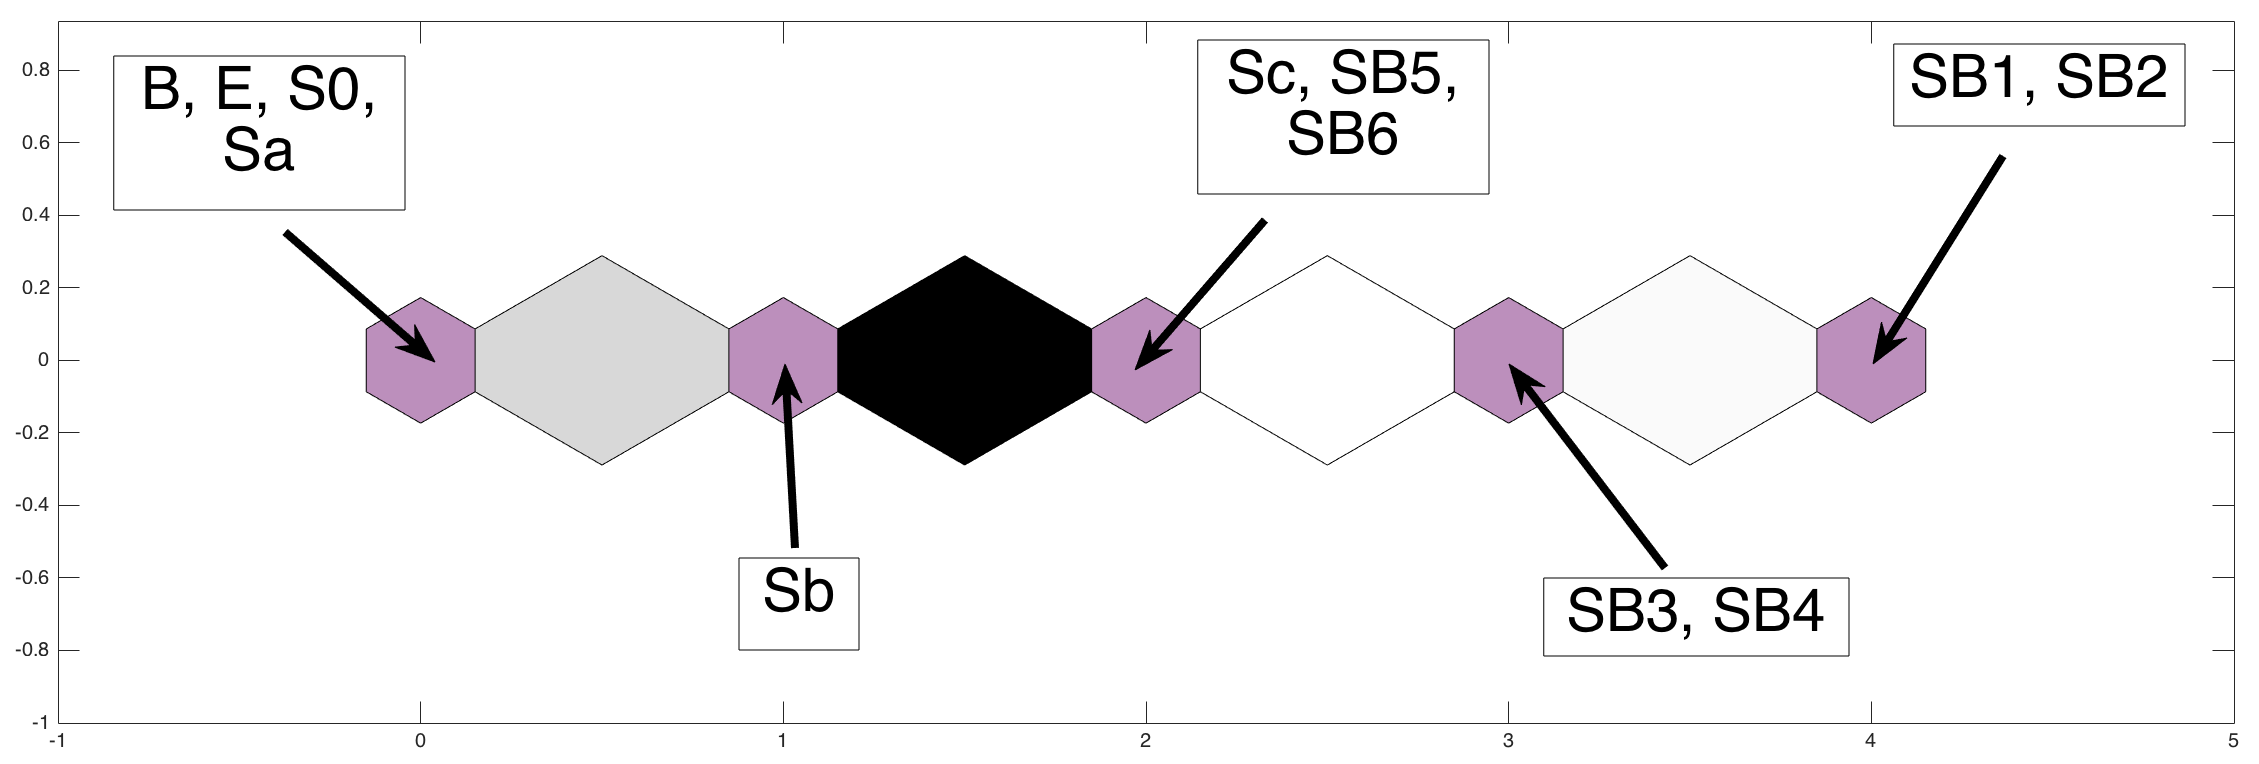
\includegraphics[width=\textwidth]{../image_paper2/1d/apps/dist_1_by_5.png}
            %\caption{$1\times5$ weight map}
             %\label{fig: 1by5T}
        \end{subfigure}
        \hfill
        \begin{subfigure}[b]{0.5\textwidth}
             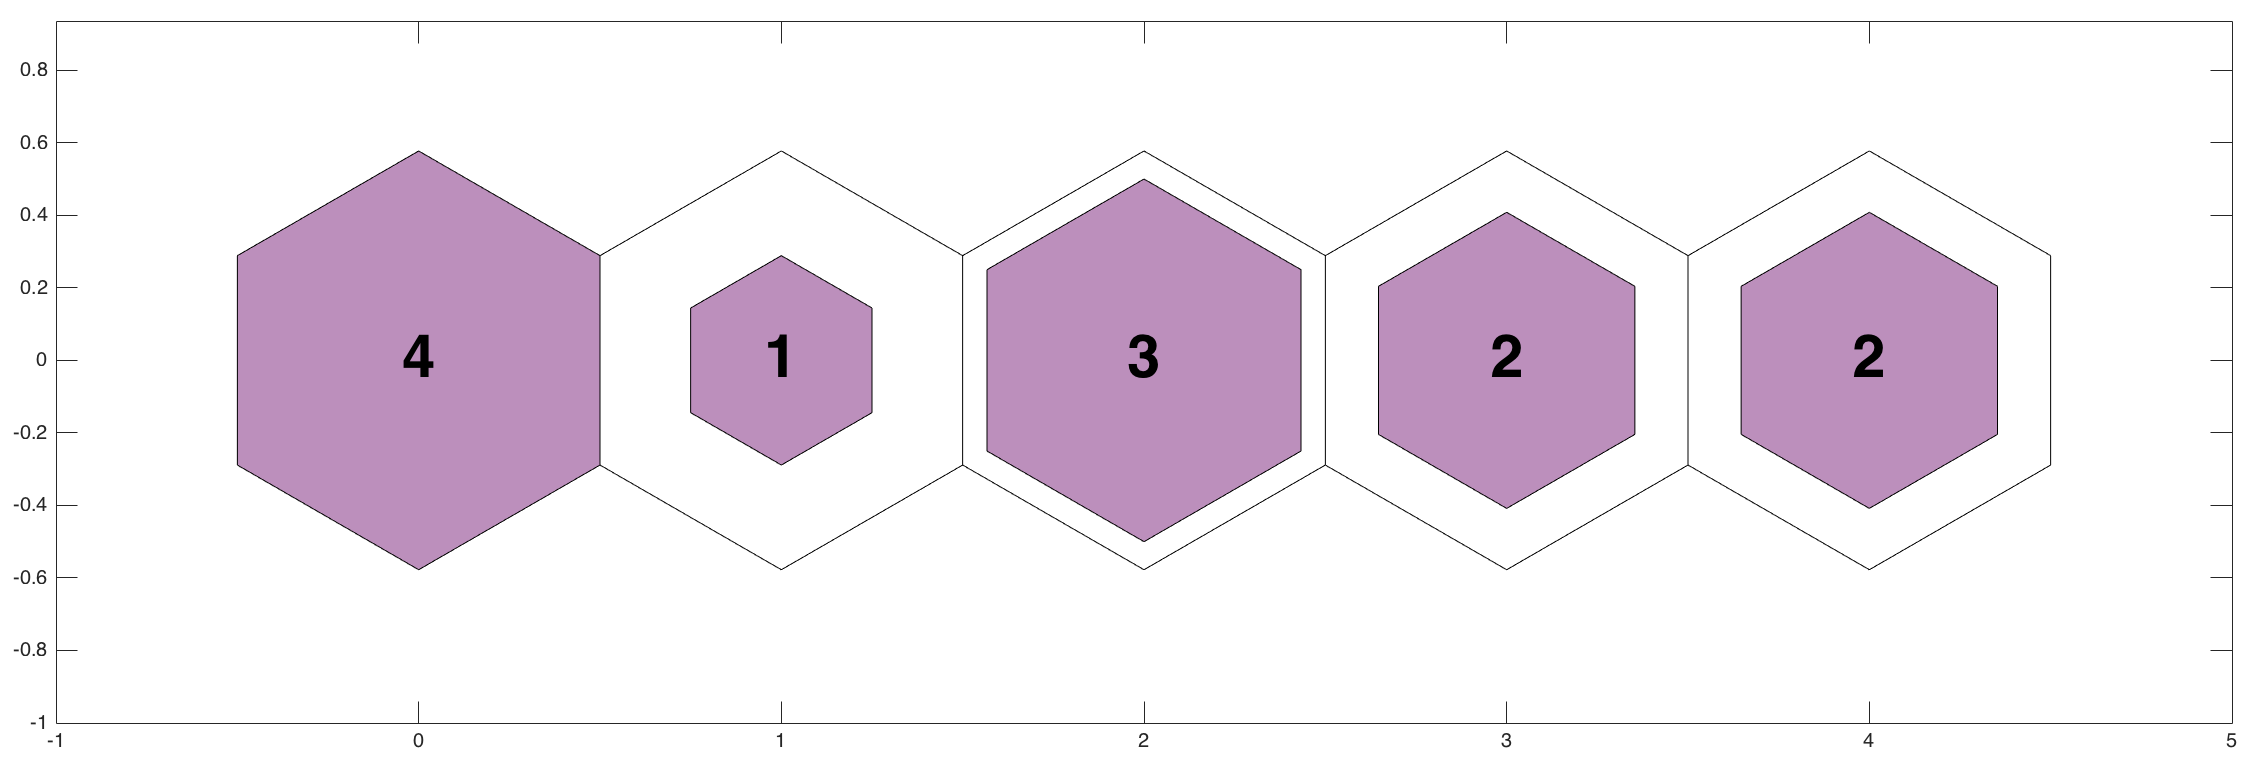
\includegraphics[width=\textwidth]{../image_paper2/1d/apps/hit_t_1_by_5.png}
             %\caption{$1\times5$ hits map}
             %\label{fig: 1by5Thits}
        \end{subfigure}
                \caption{Results of training network in $1\times5$~grid.}
         \label{fig: 1by5T}
    \end{figure}
    
    \begin{figure}
        \begin{subfigure}[b]{0.5\textwidth}
            \centering
            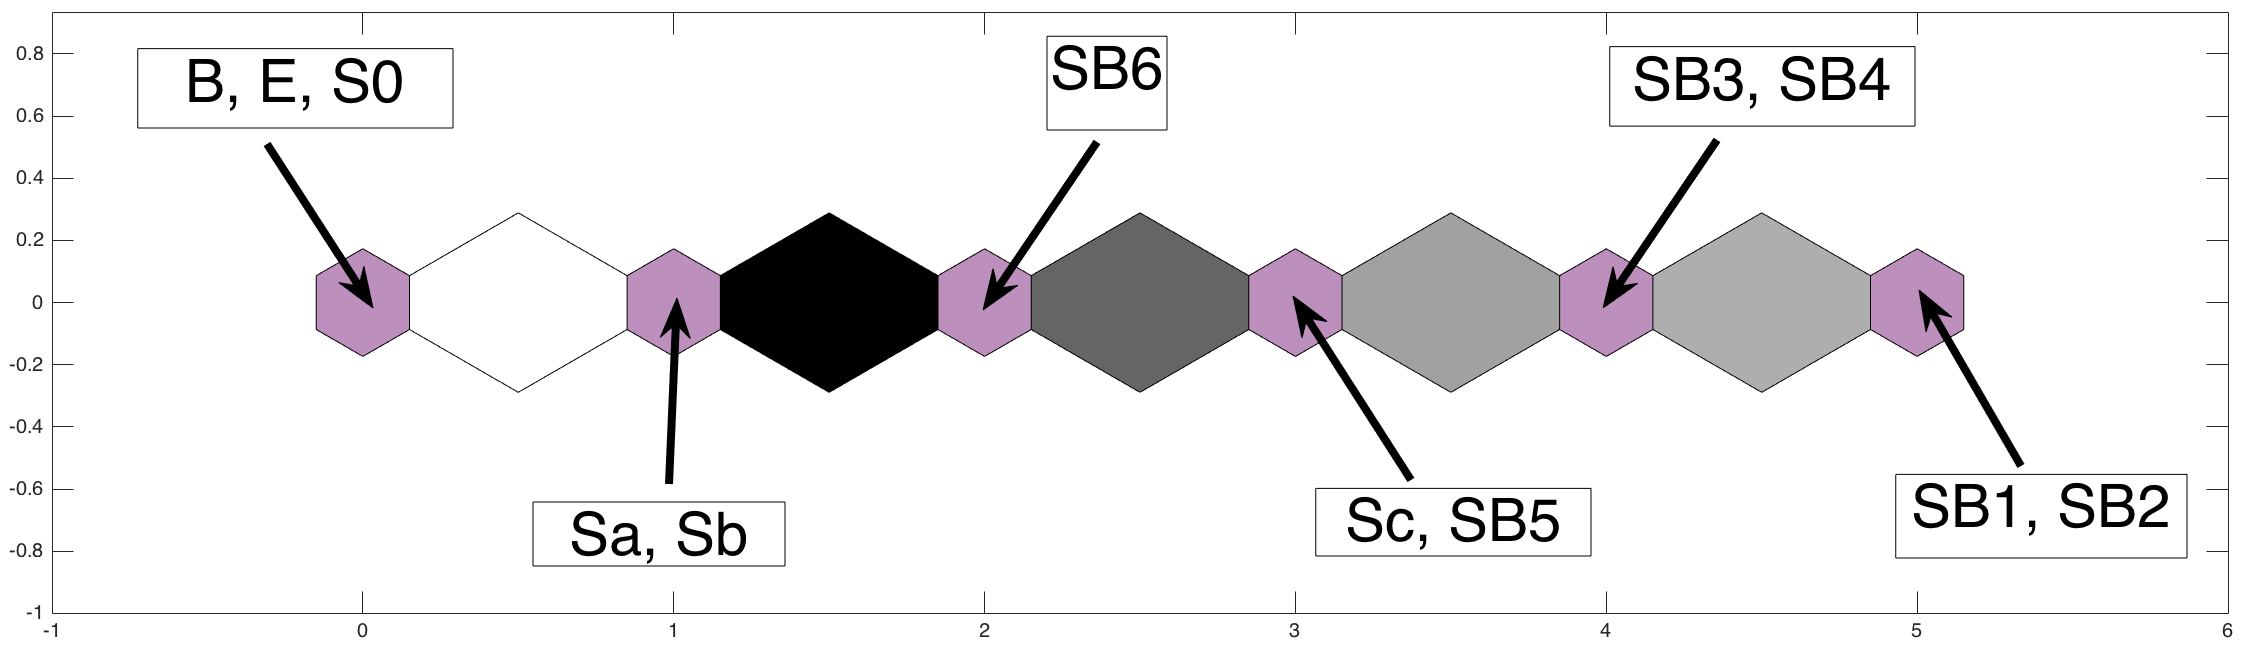
\includegraphics[width=\textwidth]{../image_paper2/1d/apps/dist_1_by_6.png}
            %\caption{$1\times6$ weight map}
             %\label{fig: 1by6T}
        \end{subfigure}
        \hfill
        \begin{subfigure}[b]{0.5\textwidth}
             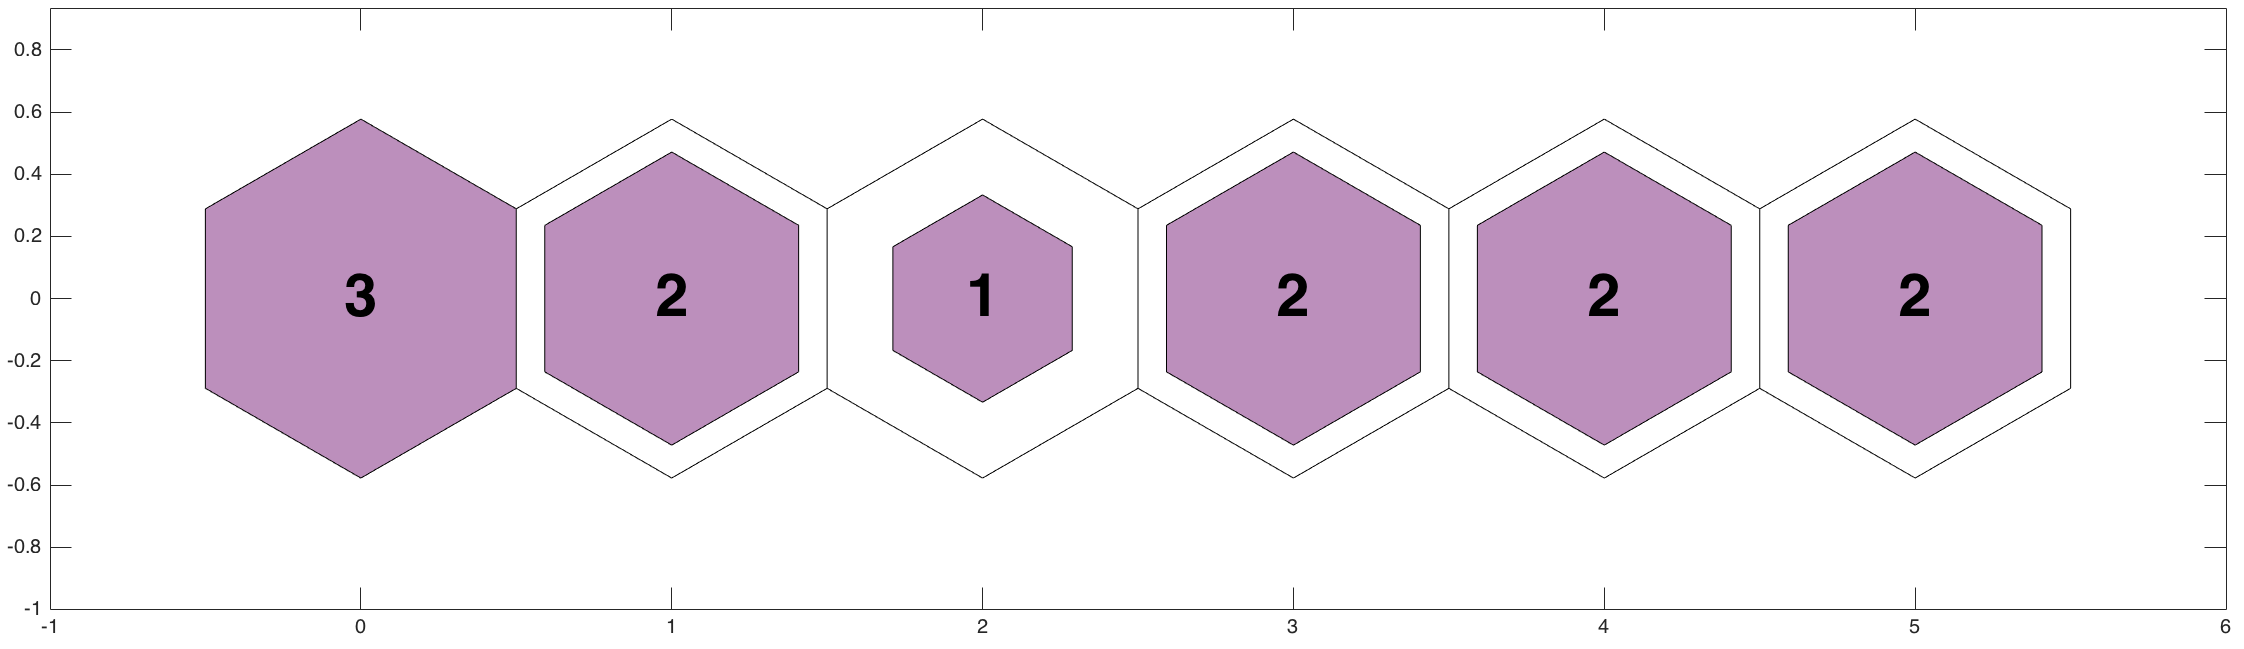
\includegraphics[width=\textwidth]{../image_paper2/1d/apps/hit_t_1_by_6.png}
             %\caption{$1\times6$ hits map}
             %\label{fig: 1by6Thits}
        \end{subfigure}
                \caption{Results of training network in $1\times6$~grid.}
         \label{fig: 1by6T}
    \end{figure}
    
    \begin{figure}
        \begin{subfigure}[b]{0.5\textwidth}
            \centering
            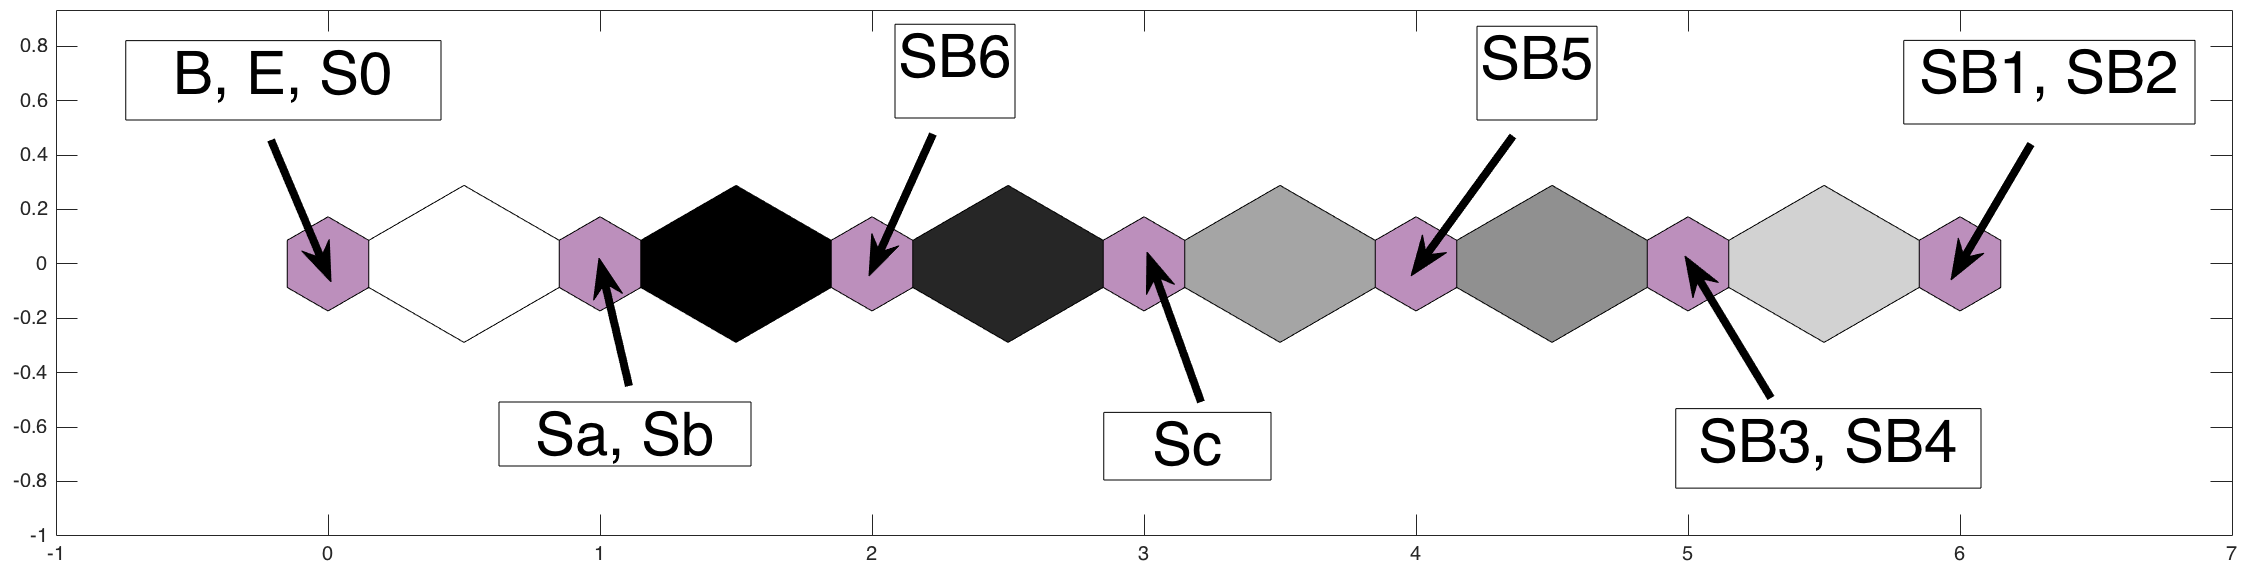
\includegraphics[width=\textwidth]{../image_paper2/1d/apps/dist_1_by_7.png}
            %\caption{$1\times7$ weight map}
             %\label{fig: 1by7T}
        \end{subfigure}
        \hfill
        \begin{subfigure}[b]{0.5\textwidth}
             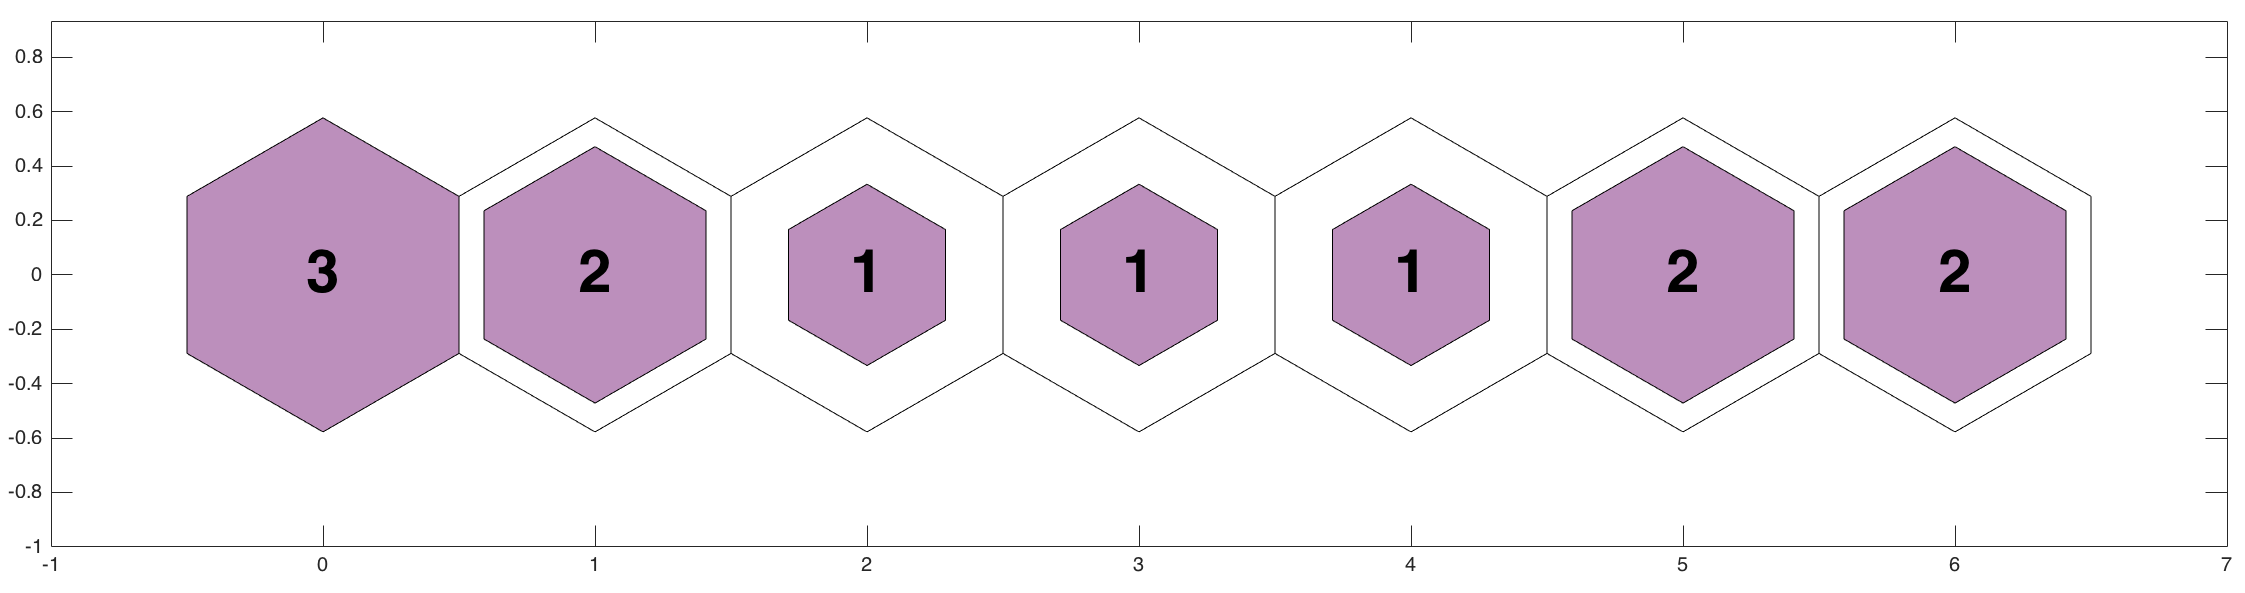
\includegraphics[width=\textwidth]{../image_paper2/1d/apps/hit_t_1_by_7.png}
             %\caption{$1\times7$ hits map}
             %\label{fig: 1by7Thits}
        \end{subfigure}
                \caption{Results of training network in $1\times7$~grid.}
         \label{fig: 1by7T}
    \end{figure}
    
    \begin{figure}
        \begin{subfigure}[b]{0.5\textwidth}
            \centering
            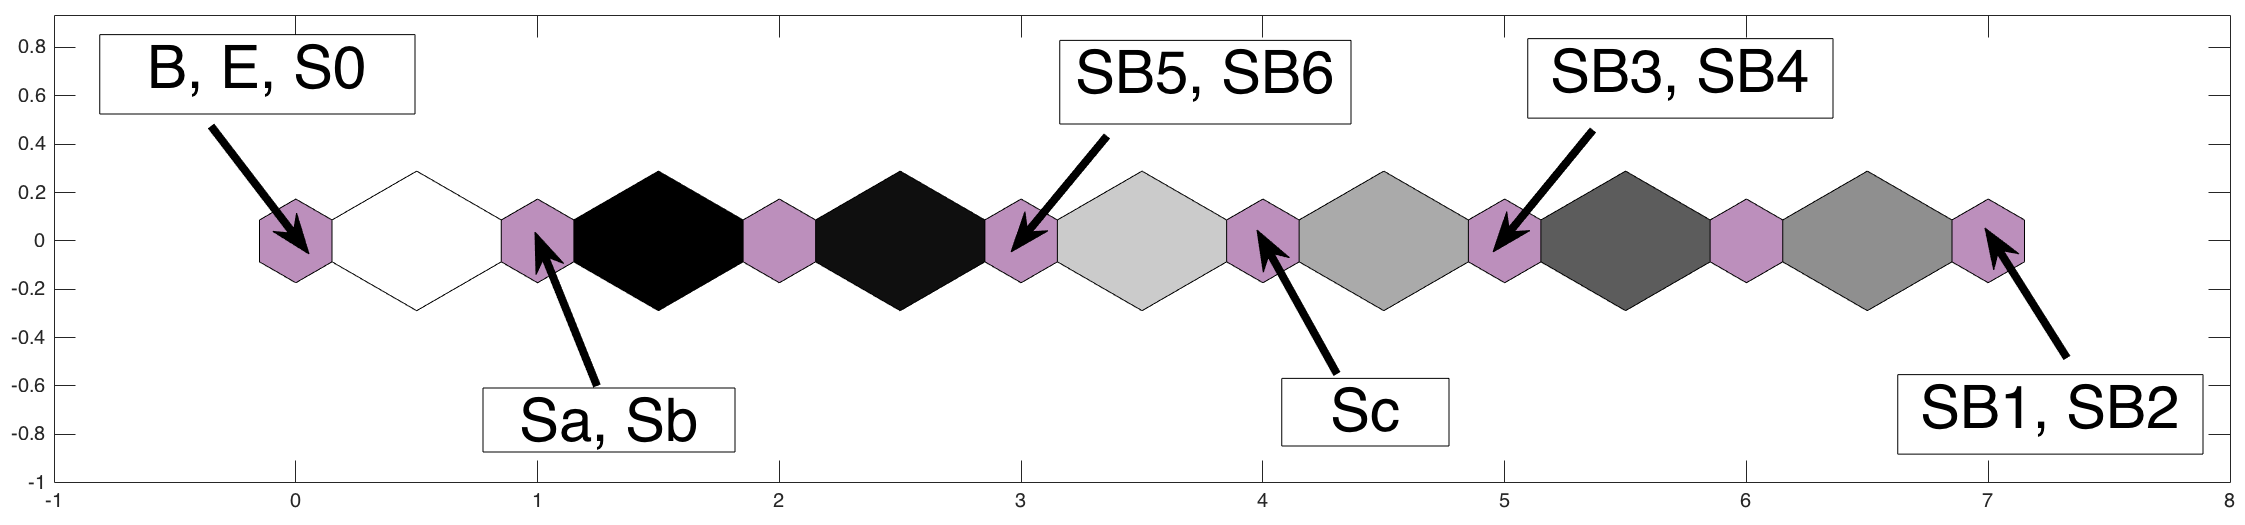
\includegraphics[width=\textwidth]{../image_paper2/1d/apps/dist_1_by_8.png}
            %\caption{$1\times8$ weight map}
             %\label{fig: 1by8T}
        \end{subfigure}
        \hfill
        \begin{subfigure}[b]{0.5\textwidth}
             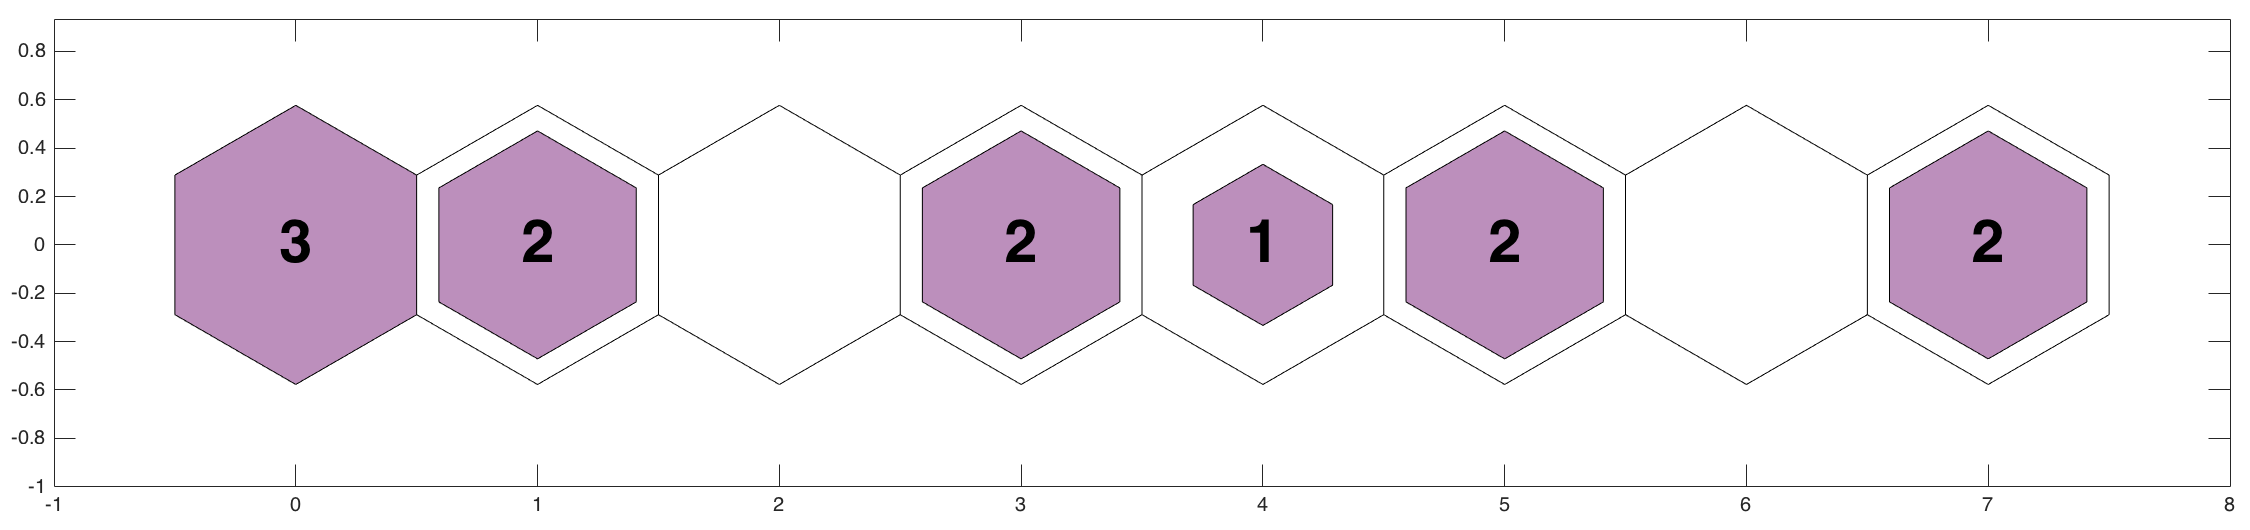
\includegraphics[width=\textwidth]{../image_paper2/1d/apps/hit_t_1_by_8.png}
             %\caption{$1\times8$ hits map}
             %\label{fig: 1by8Thits}
        \end{subfigure}
                \caption{Results of training network in $1\times8$~grid.}
         \label{fig: 1by8T}
    \end{figure}
    
    \begin{figure}
        \begin{subfigure}[b]{0.5\textwidth}
            \centering
            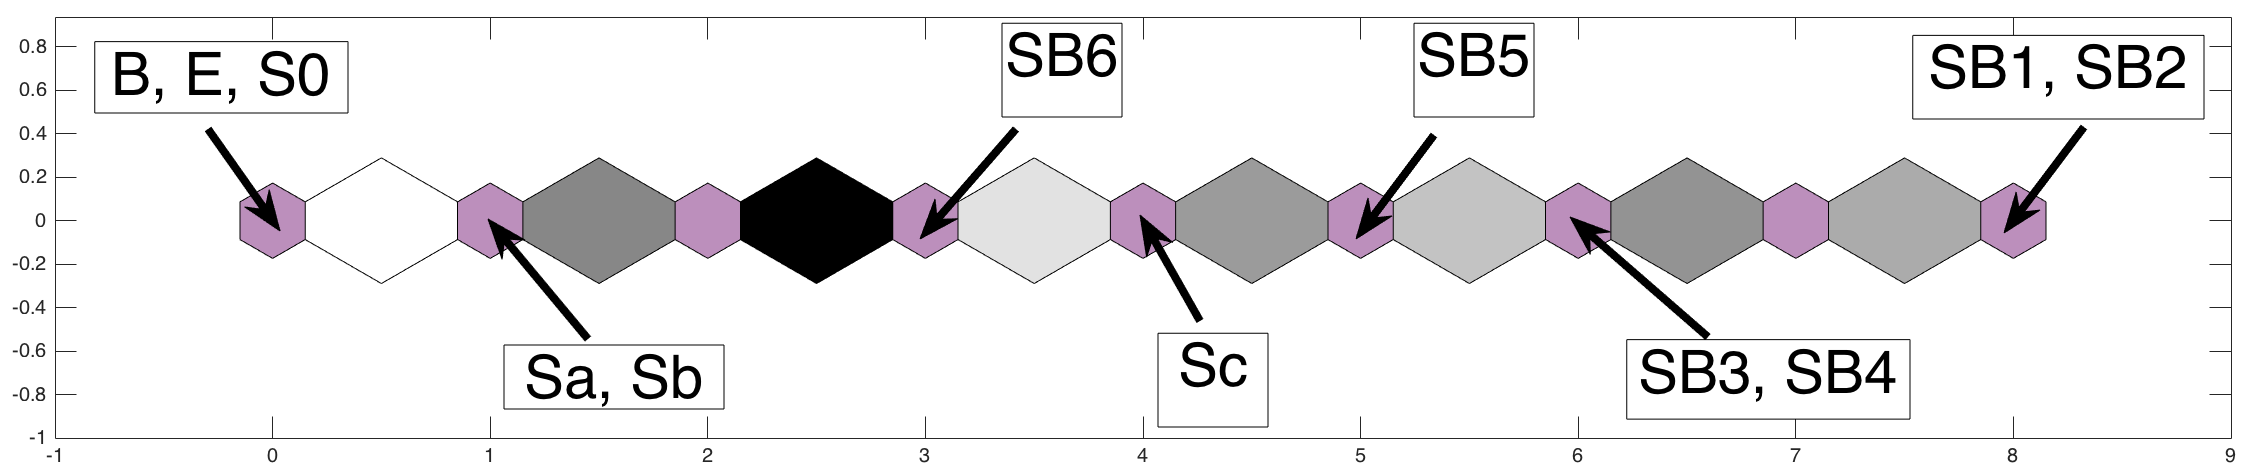
\includegraphics[width=\textwidth]{../image_paper2/1d/apps/dist_1_by_9.png}
            %\caption{$1\times9$ weight map}
             %\label{fig: 1by9T}
        \end{subfigure}
        \hfill
        \begin{subfigure}[b]{0.5\textwidth}
             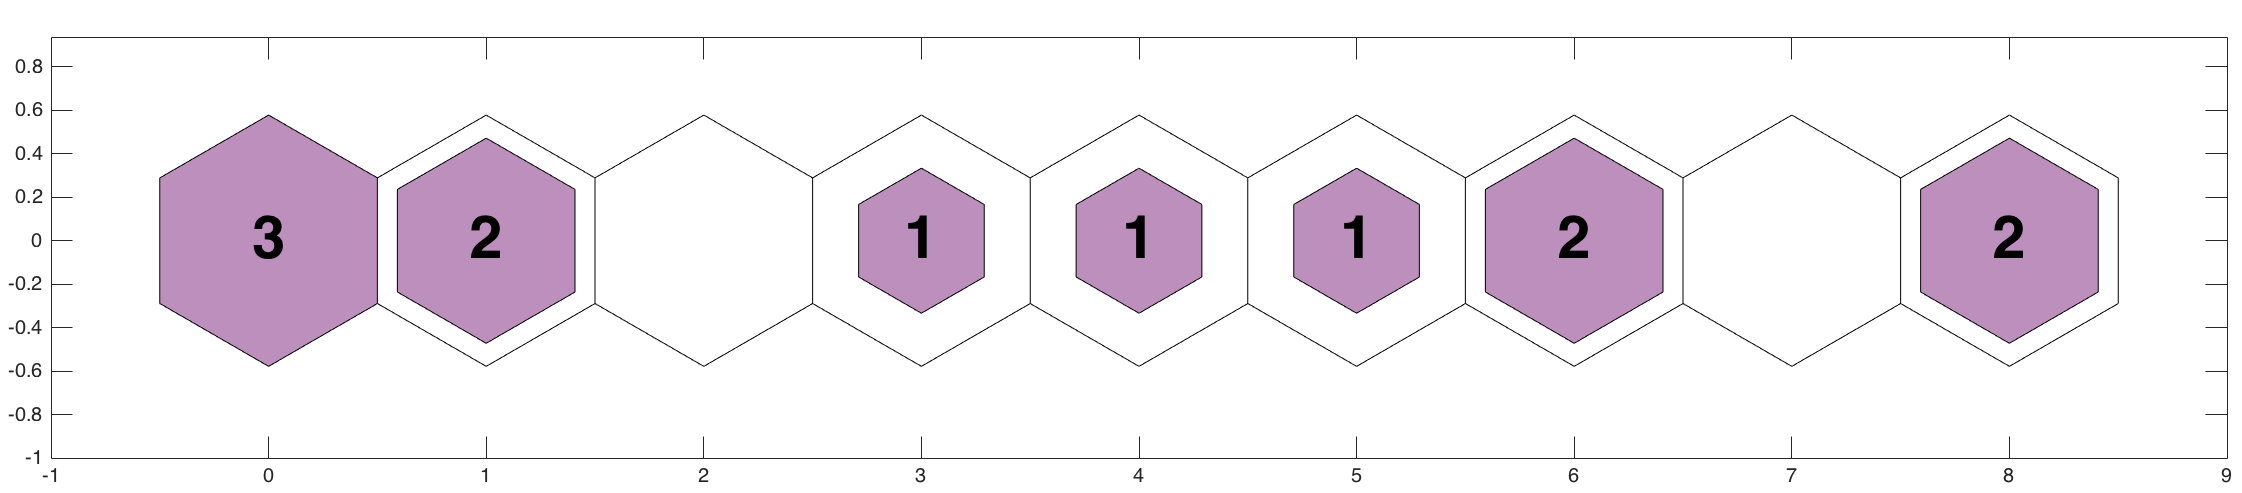
\includegraphics[width=\textwidth]{../image_paper2/1d/apps/hit_t_1_by_9.png}
             %\caption{$1\times9$ hits map}
             %\label{fig: 1by9Thits}
        \end{subfigure}
                \caption{Results of training network in $1\times9$~grid.}
         \label{fig: 1by9T}
    \end{figure}

    \begin{figure}
        \begin{subfigure}[b]{0.5\textwidth}
            \centering
            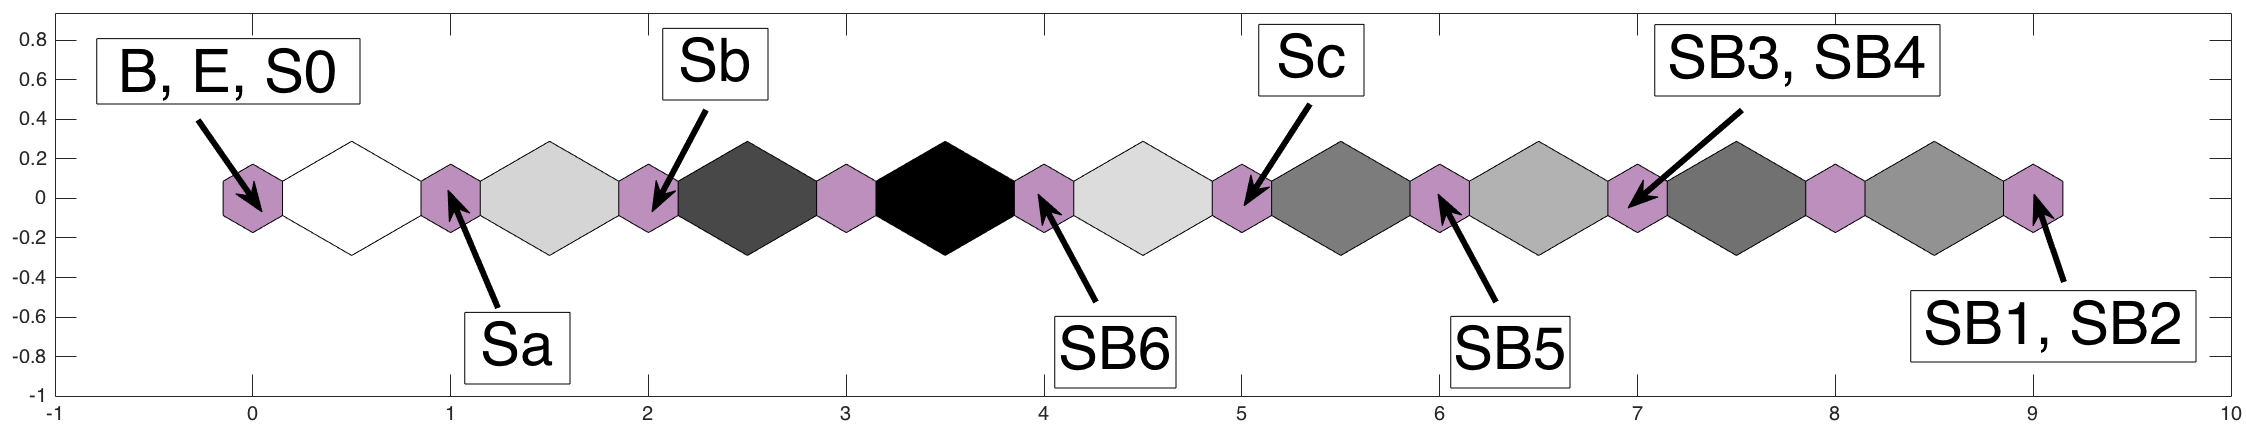
\includegraphics[width=\textwidth,height=2.5cm]{../image_paper2/1d/apps/dist_1_by_10.png}
            %\caption{$1\times10$ weight map}
             %\label{fig: 1by10T}
        \end{subfigure}
        \hfill
        \begin{subfigure}[b]{0.5\textwidth}
             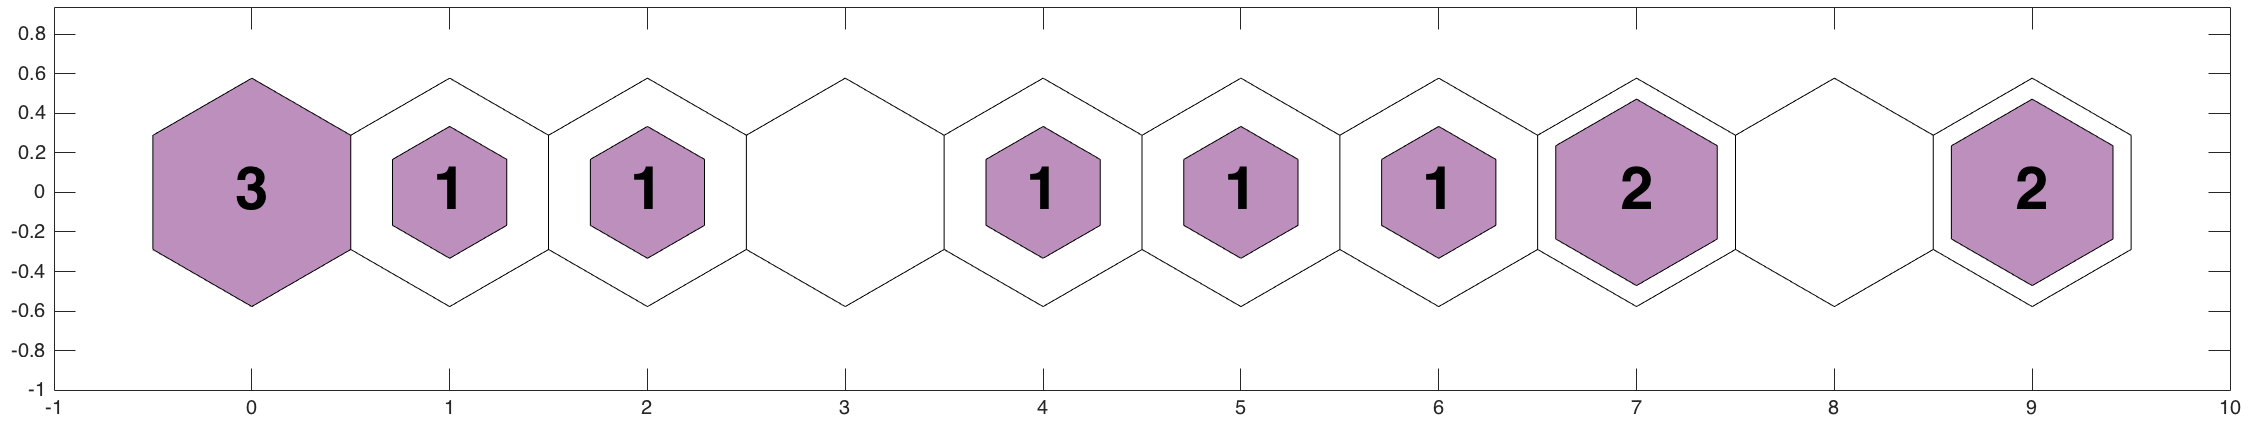
\includegraphics[width=\textwidth,height=2.5cm]{../image_paper2/1d/apps/hit_t_1_by_10.png}
             %\caption{$1\times10$ hits map}
             %\label{fig: 1by10Thits}
        \end{subfigure}
                \caption{Results of training network in $1\times10$~grid.}
         \label{fig: 1by10T}
    \end{figure}

    \begin{figure}
        \begin{subfigure}[b]{0.5\textwidth}
            \centering
            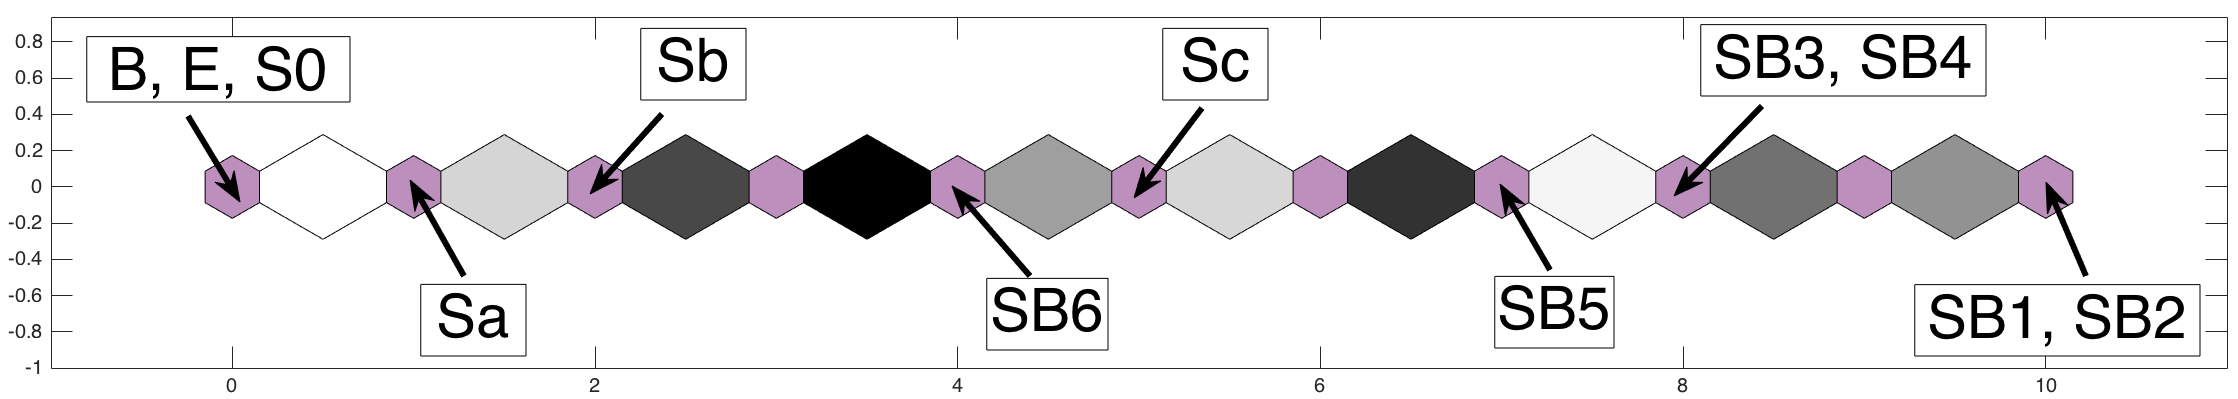
\includegraphics[width=\textwidth,height=2.5cm]{../image_paper2/1d/apps/dist_1_by_11.png}
            %\caption{$1\times11$ weight map}
             %\label{fig: 1by11T}
        \end{subfigure}
        \hfill
        \begin{subfigure}[b]{0.5\textwidth}
             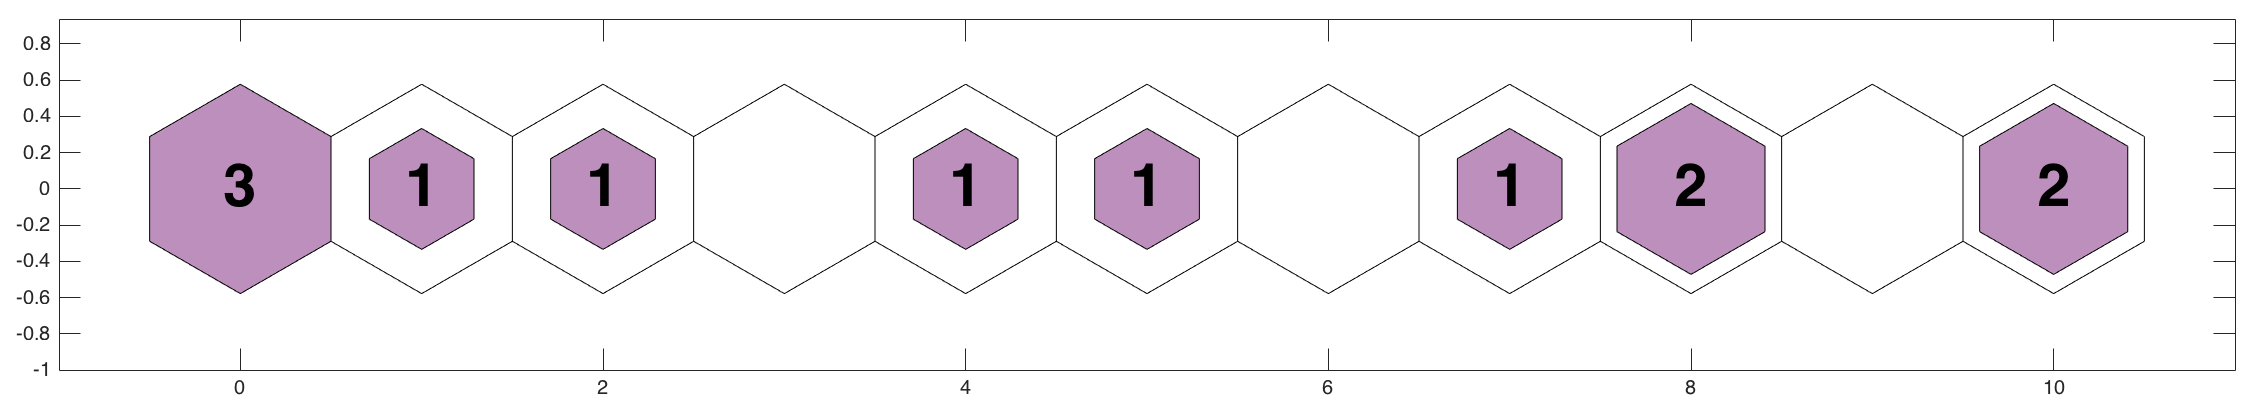
\includegraphics[width=\textwidth,height=2.5cm]{../image_paper2/1d/apps/hit_t_1_by_11.png}
             %\caption{$1\times11$ hits map}
             %\label{fig: 1by11Thits}
        \end{subfigure}
                \caption{Results of training network in $1\times11$~grid.}
         \label{fig: 1by11T}
    \end{figure}
    

    \begin{figure}
        \begin{subfigure}[b]{0.5\textwidth}
            \centering
            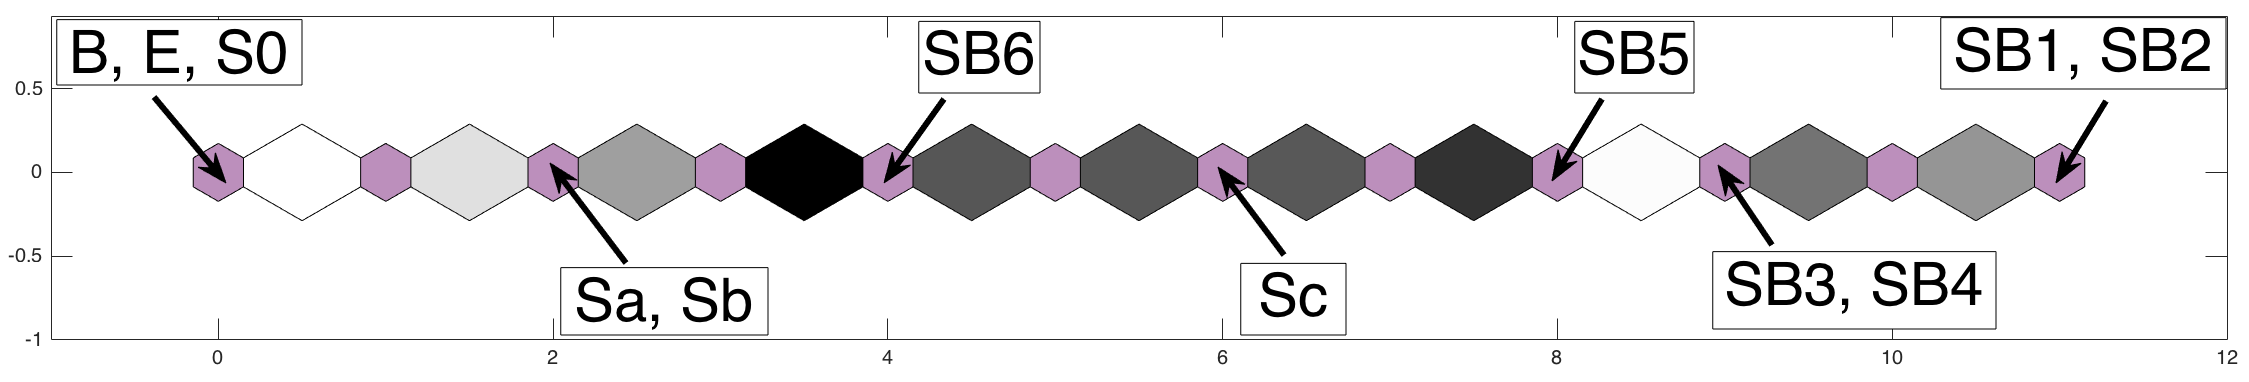
\includegraphics[width=\textwidth,height=2.5cm]{../image_paper2/1d/apps/dist_1_by_12.png}
            %\caption{$1\times12$ weight map}
             %\label{fig: 1by12T}
        \end{subfigure}
        \hfill
        \begin{subfigure}[b]{0.5\textwidth}
             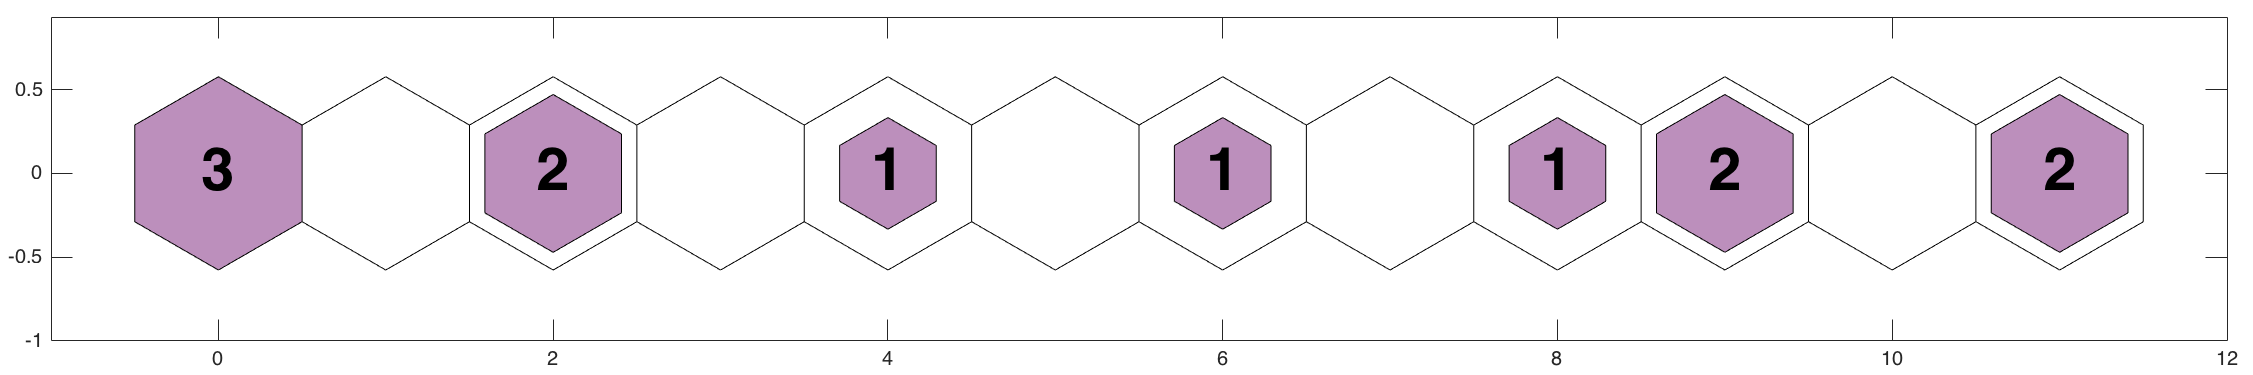
\includegraphics[width=\textwidth,height=2.5cm]{../image_paper2/1d/apps/hit_t_1_by_12.png}
             %\caption{$1\times12$ hits map}
             %\label{fig: 1by12Thits}
        \end{subfigure}
                \caption{Results of training network in $1\times12$~grid.}
         \label{fig: 1by12T}
    \end{figure}

    \begin{figure}
        \begin{subfigure}[b]{0.5\textwidth}
            \centering
            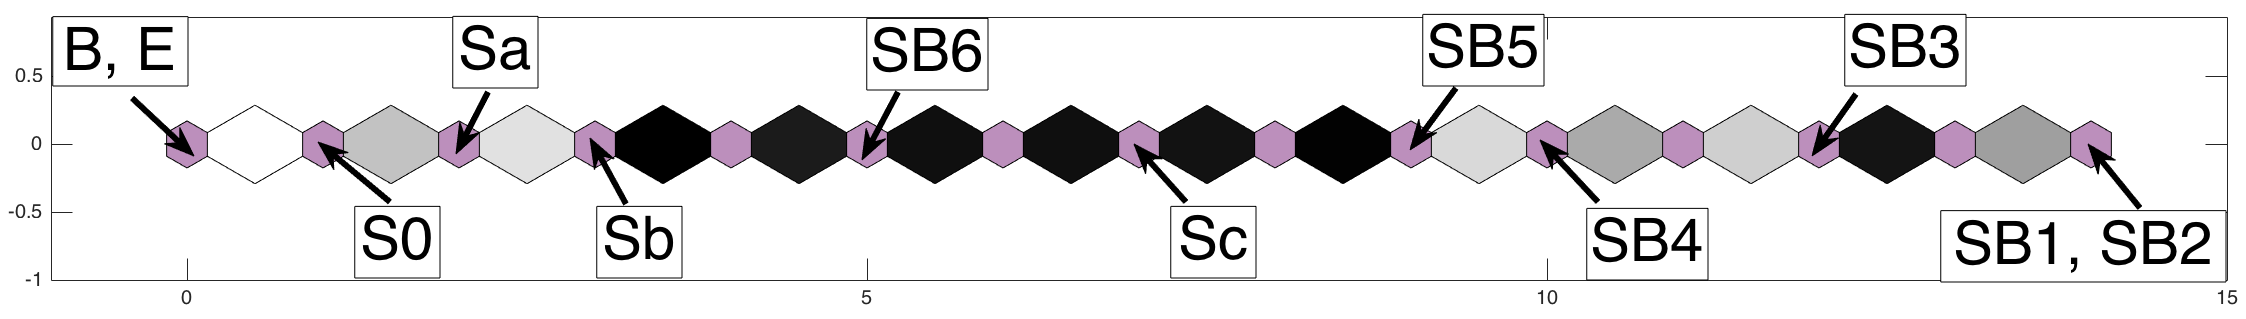
\includegraphics[width=\textwidth,height=2.5cm]{../image_paper2/1d/apps/dist_1_by_15.png}
            %\caption{$1\times15$ weight map}
             %\label{fig: 1by15T}
        \end{subfigure}
        \hfill
        \begin{subfigure}[b]{0.5\textwidth}
             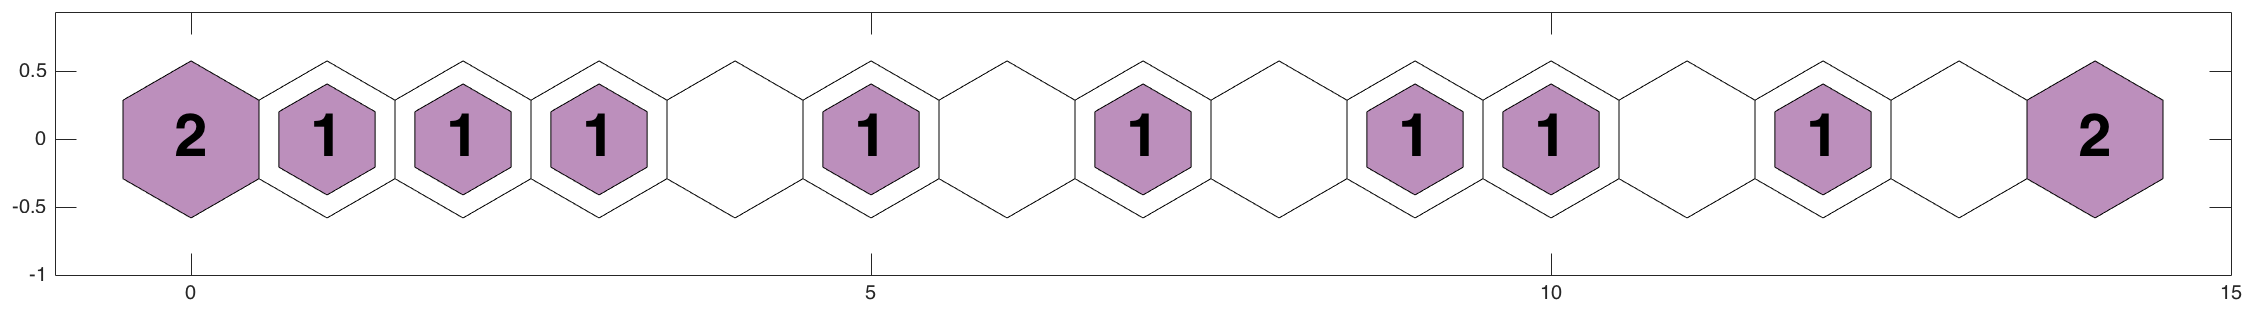
\includegraphics[width=\textwidth,height=2.5cm]{../image_paper2/1d/apps/hit_t_1_by_15.png}
             %\caption{$1\times15$ hits map}
             %\label{fig: 1by15Thits}
        \end{subfigure}
                \caption{Results of training network in $1\times15$~grid.}
         \label{fig: 1by15T}
    \end{figure}

    \begin{figure}
        \begin{subfigure}[b]{0.5\textwidth}
            \centering
            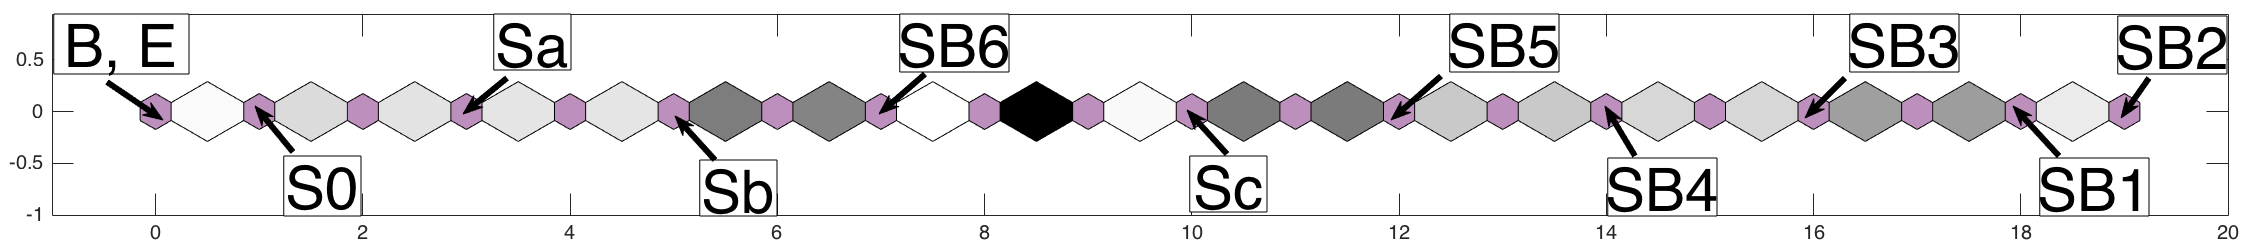
\includegraphics[width=\textwidth,height=2.5cm]{../image_paper2/1d/apps/dist_1_by_20.png}
            %\caption{$1\times20$ weight map}
             %\label{fig: 1by20T}
        \end{subfigure}
        \hfill
        \begin{subfigure}[b]{0.5\textwidth}
             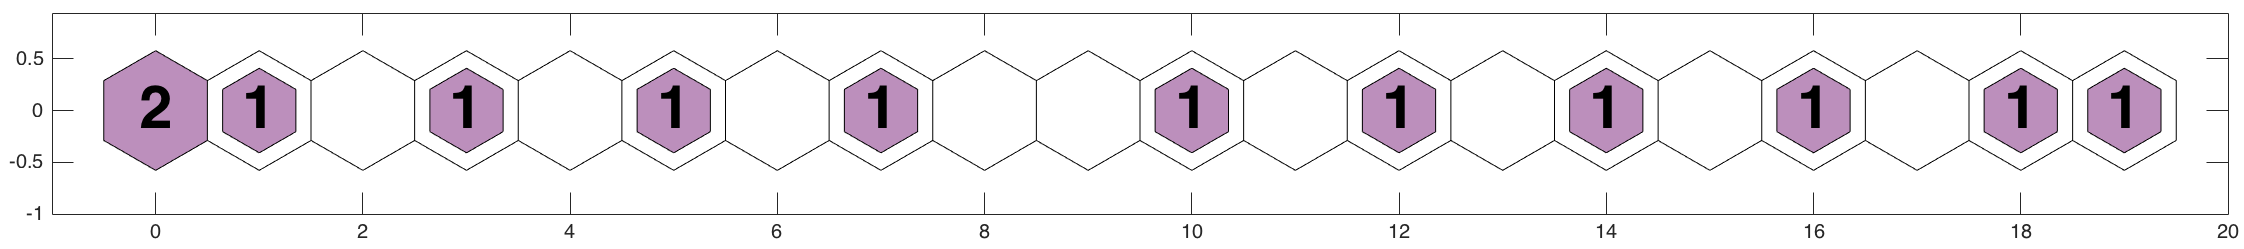
\includegraphics[width=\textwidth,height=2.5cm]{../image_paper2/1d/apps/hit_t_1_by_20.png}
             %\caption{$1\times20$ hits map}
             %\label{fig: 1by20Thits}
        \end{subfigure}
                \caption{Results of training network in $1\times20$~grid.}
         \label{fig: 1by20T}
    \end{figure}
    